\documentclass{article}

\usepackage[T1]{fontenc} % encodage
\usepackage[french]{babel}
\usepackage[hidelinks]{hyperref} % liens cliquable dans la table des matières
\usepackage{minted} % intégration code
\usepackage{graphicx} % images

\usemintedstyle{emacs}

\renewcommand{\familydefault}{\sfdefault} % police en "sans-serif"

\renewcommand{\contentsname}{Table des matières} % traduction en FR

\title{\href{https://code.up8.edu/Anri/bomberman}{Bomberman}}
\author{Anri Kennel\thanks{Numéro d'étudiant : 20010664}\, (L2-A)\\APG $\cdot$ Paris 8}
\date{Année universitaire 2021-2022}

\begin{document}
    \maketitle
    \tableofcontents
    \clearpage

    \section{Base}
    Je suis partie du projet du \href{https://expreg.org/amsi/C/APG2122S1/code/sc_00_07_rasterizer-0.1.tgz}{\underline{rasterizer DIY}}
    donné avec le \href{https://expreg.org/amsi/C/APG2122S1/code/S9GB/MODIF1/window.c}{\underline{fichier \texttt{window.c}}} de la semaine 9 Groupe B
    pour avoir une base pour le plateau de jeu ainsi que pour le personnage.
    J'ai apporté aucune modifications au rasterizer.

    \section[Présentation]{Brève présentation}
    J'ai réalisé le projet seul. Mon projet est le bomberman en vue isométrique.

    \begin{figure}[!ht]
        \centering
        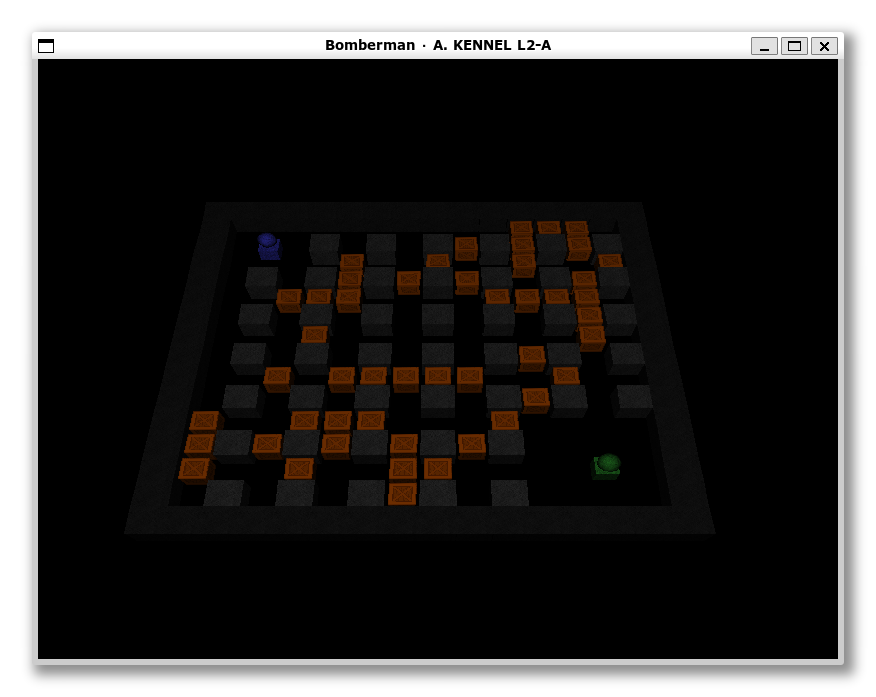
\includegraphics[height=0.49\textheight]{game.png}
        \caption{Nouvelle partie}
    \end{figure}

    \subsection[Objectif et réalisation]{\href{https://expreg.org/amsi/C/APG2122S1/supports/projets.pdf}{Objectif et réalisation}}
    \begin{itemize}
        \item Sur la base d’un générateur de labyrinthes, modéliser aléatoirement chaque nouveau niveau : on pourra utiliser différents types de cubes
        comme dans le jeu original
        \begin{itemize}
            \item Cette objectif a été remplie
            \item Des cubes noir entoure le plateau de jeu
            \item Des blocs gris parsème l'intérieur du plateau
            \item Des blocs marrons avec une texture différente représente les blocs cassable par les joueurs et sont placés aléatoirement sur le plateau
        \end{itemize}

        \item Les joueurs seront simplement modélisés par un cône surmonté d’une sphère, et couleurs différentes ; des sphères noires pour les bombes ; des sphères jaunes dont rayon décroit jusqu’à disparaître pour les effet d’explosion ...
        \begin{itemize}
            \item Cette objectif a été partiellement réalisé
            \item Les joueurs sont modélisés avec des cubes surmonté d'une sphère
            \item Les joueurs sont de couleurs différentes (bleu et vert)
            \item Les bombes sont représentés par des sphères qui varie du marron au rouge en passant par l'orange en fonction du temps restant avec explosion
            \item La taille de la bombe ne varie que lors de la dernière demi-seconde pour un effet "bombe atomique" qui explose sous forme d'un cercle grossissant lors de ces derniers instants
        \end{itemize}

        \item Gérer toutes les collisions et intéractions liées au jeu
        \begin{itemize}
            \item Cette objectif a été réalisé
            \item Les joueurs sont bloqués par les murs, les autres joueurs et les bombes des autres joueurs
        \end{itemize}

        \item Gérer l’IA des autres joueurs
        \begin{itemize}
            \item Cette objectif n'a pas été réalisé
        \end{itemize}

        \item Gérer un mode multi-joueurs "humains" sur le même poste
        \begin{itemize}
            \item Cette objectif a été réalisé
            \item Le joueur vert contrôle son personnage avec les flèches directionnelles et pose sa bombe avec la touche \texttt{Entrée}
            \item Le joueur bleu contrôle son personnage avec les touches \texttt{Z Q S D} et pose sa bombe avec la \texttt{barre espace}
        \end{itemize}

        \item Gérer un mode multi-joueurs "humains" en réseau
        \begin{itemize}
            \item Cette objectif n'a pas été réalisé
        \end{itemize}
    \end{itemize}

    \section[Explication]{Explication de la réalisation}
    Dans mon code, le joueur A représente le joueur vert et le joueur B est le joueur bleu.
    \vspace{10pt}

    J'active par défaut les textures et les ombrages sur tous les objets, ainsi que la synchronisation verticale.
    \vspace{10pt}

    La structure du joueur est composé des coordonnées spatiale \texttt{x, y, z} ainsi que sa position dans le plateau, l'heure à laquelle sa dernière bombe (\texttt{0} quand pas de bombe) à été posée et la position de sa bombe (\texttt{-1} quand pas de bombe)
    \begin{center}\begin{minipage}{0.5\textwidth}
        \begin{minted}[linenos]{c}
typedef struct perso_t {
    float x, y, z;
    int position;
    double bombe;
    int bombePos;
} perso_t;
        \end{minted}
    \end{minipage}\end{center}
    \vspace{10pt}

    Les dimensions du plateau sont choisies aléatoirement mais le plateau est toujours un carré. Les dimensions varient entre \texttt{15} et \texttt{25} cube de côté.
    \begin{center}\begin{minipage}{0.5\textwidth}
        \begin{minted}[linenos]{c}
srand(time(NULL));
_plateauW = 15 + (rand() % 10);
_plateauH = _plateauW;
        \end{minted}
    \end{minipage}\end{center}
    \vspace{10pt}

    Les joueurs sont placés de façon à être éloignés l'un de l'autre. Le joueur A est placé en bas à gauche du plateau et le joueur B en haut à droite.
    \begin{center}\begin{minipage}{0.8\textwidth}
        \begin{minted}[linenos]{c}
/* Joueur A */
int caseA = (_plateauW * _plateauH) - (_plateauW * 2) - 3;
_joueurA.x = (caseA / _plateauH) * 1.5;
_joueurA.z = (caseA / _plateauW) * 1.5;

/* Joueur B */
int caseB = (_plateauW * 2) + 3;
_joueurB.x = -(caseB / _plateauH) * 12;
_joueurB.z = -(caseB / _plateauW) * 12;
        \end{minted}
    \end{minipage}\end{center}
    \vspace{10pt}

    En accord avec les dimensions du plateau, il faut aussi changer la position de la caméra. Elle doit être proche quand le plateau est petit et éloigné quand le plateau est grand.
    \begin{center}\begin{minipage}{0.5\textwidth}
        \begin{minted}[linenos]{c}
int coefTaille = -20 + _plateauW * 2.5;
lookAt(
    model_view_matrix, 0,
    70 + coefTaille,  // zoom
    30 + coefTaille , // inclinaison
    0, 0, 0, 0, 0, -1);
        \end{minted}
    \end{minipage}\end{center}
    \vspace{10pt}

    Les alentours des joueurs est vidé, c'est-à-dire que il n'y a pas de blocs aux alentour du joueur pour éviter qu'ils apparaissent dans un mur (déstructible ou non)
    \vspace{10pt}

    La grille du plateau est composé de chiffres allant de \texttt{0} à \texttt{7} :
    \begin{itemize}
        \item 0 représente du vide
        \item 1 représente un mur
        \item 2 représente le Joueur A
        \item 3 représente le Joueur B
        \item 4 représente un mur destructible
        \item 5 représente la bordure extérieure
        \item 6 représente la bombe du joueur A
        \item 7 représente la bombe du joueur B
    \end{itemize}
    \vspace{10pt}

    Les collisions sont gérées grâce à la grille, lorsque l'on essaie de se déplacer, on vérifie qu'il n'y a pas de cube là où on veut aller. Pour cela on calcule la position des blocs à gauche, à droite, au-dessus et en dessous du joueur.
    \begin{center}\begin{minipage}{0.9\textwidth}
        \begin{minted}[linenos]{c}
/* Exemple vérification pour aller à droite pour le joueur A
 * _cubeSize est la taille du cube */
float zA = (_joueurA.z + _cubeSize * _plateauH / 2) / _cubeSize;
float xA = (_joueurA.x + _cubeSize * _plateauW / 2) / _cubeSize;
int posDroiteA = round(zA) * _plateauH + ceil(xA);
if(_vkeyboard[VK_RIGHT])
    if( _plateau[posDroiteA] == 0 || // si vide
        _plateau[posDroiteA] == 2 || // si joueur
        _plateau[posDroiteA] == 6)   // si bombe-joueur
            _joueurA.x += vitesse * dt;
        \end{minted}
    \end{minipage}\end{center}
    \vspace{10pt}

    Comme dit ci-dessus, la collision est gérée grâce à la grille, alors les joueurs doivent aussi être dans la grille, même s'il se déplace de façon fluide. A chaque fois que le centre de gravité du joueur change de case, son numéro change aussi de case dans la grille.
    \vspace{10pt}

    La bombe est rattachée au joueur et il n'y peut y avoir qu'une bombe à la fois par joueur sur le terrain. Ces informations sont stockées dans la structure du joueur. \texttt{bombe} correspond à l'heure où la bombe a été posée sur le terrain et \texttt{bombePos} est la position de la bombe sur la grille.
    Une bombe reste 3 secondes sur le terrain. La première seconde elle est marron, puis elle devient orange au bout de la 2\up{ème} seconde. A partir de la 3\up{ème} seconde elle devient rouge et une demi-seconde plus tard elle grossit soudainement, puis grossit encore progressivement pendant une dernière demi-seconde avant de disparaître en supprimant les cubes "en bois" qui était dans son rayon. Elle arrête aussi la partie si un joueur a été touché par le rayon de l'explosion et le résultat est affiché dans le terminal.
    Le programme détecte les cubes grâce à la grille :
    \begin{center}\begin{minipage}{0.9\textwidth}
        \begin{minted}[linenos]{c}
/* Exemple détection si un cube est dans le rayon de
 * l'explosion dans un rayon i dans la direction vers le haut
 * à gauche (4 signifie que le cube destructible) */
if(_plateau[_joueurA.bombePos - _plateauW - i] == 4)
    _plateau[_joueurA.bombePos - _plateauW - i] = 0;
        \end{minted}
    \end{minipage}\end{center}

    En revanche, la détection des joueurs est différente, on ne peut pas se fier à la grille car si un joueur pose une bombe et reste à l'emplacement de cette dernière, sur la grille, il n'y aura pas le joueur à la position du joueur mais la bombe. On se base donc sur sa position en temps réel et non par le biais du plateau.
    \begin{center}\begin{minipage}{0.9\textwidth}
        \begin{minted}[linenos]{c}
/* Vérification mort d'un joueur */
/* Si position joueur = position bombe
 * (on vérifie pour les deux joueurs) */
if(_joueurA.bombePos == posJoueurA) trouveA = 1;
if(_joueurA.bombePos == posJoueurB) trouveB = 1;
        \end{minted}
    \end{minipage}\end{center}
    \vspace{10pt}

    Les objets 3D sont dessinés dans la méthode \texttt{draw()} :
    \begin{center}\begin{minipage}{0.9\textwidth}
        \begin{minted}[linenos]{c}
/* Exemple dessin du joueur A */
vec4 couleurJoueurA = {0.15, 0.5, 0.15, 1}; // Vert

/* On assigne au cube et à la sphère les couleurs du joueur A */
_cube->dcolor = couleurJoueurA;
_sphere->dcolor = couleurJoueurA;
memcpy(nmv, model_view_matrix, sizeof(nmv));
/* Corps */
translate(nmv, _joueurA.x, _joueurA.y, _joueurA.z);
scale(nmv, _cubeSize / 3.f, _cubeSize / 3.f, _cubeSize / 3.f);
transform_n_rasterize(_cube, nmv, projection_matrix);
/* Tête */
translate(nmv, 0.f, 2.f, 0.f);
transform_n_rasterize(_sphere, nmv, projection_matrix);
        \end{minted}
    \end{minipage}\end{center}
    \vspace{10pt}

    Les touches sont gérés grâce aux méthodes \texttt{keyd} (quand une touche est pressée) et \texttt{keyu} (quand une touche n'est plus pressée) avec une \texttt{enum} qui répertorie les touches utilisés et une liste qui garde l'état des touches (si elle est actuellement pressée ou non)
    \begin{center}\begin{minipage}{0.9\textwidth}
        \begin{minted}[linenos]{c}
/* Exemple */
enum {
    VK_RIGHT    = 0,
    VK_UP,     // 1
    VK_LEFT,   // 2
    VK_DOWN,   // 3
    VK_RETURN, // 4

    VK_SIZEOF
};                        /* Correspondance :
                           * 0  1  2  3  4 */
int _vkeyboard[VK_SIZEOF] = {0, 0, 0, 0, 0};

// Plus loin...
void keyd(int keycode) {
    switch(keycode) {
        case GL4DK_RIGHT: /* Gestion que de la flèche
                           * vers la droite pour
                           * l'exemple. */
            _vkeyboard[VK_RIGHT] = 1;
            break;

        default: break; // ne fais rien
    }
}
        \end{minted}
    \end{minipage}\end{center}
    \vspace{10pt}

    A la sortie du programme on libère tous nos éléments de la mémoire.

    \section{Ajouts}
    Possibilité d'activer ou non la synchronisation verticale ainsi de faciliter les tests de performance lorsque la touche \texttt{v} est pressée.

    \subsection{Piste d'amélioration}
    J'aurais aimé pouvoir modéliser les joueurs avec un cône au lieu d'un simple cube pour le corps.

\end{document}
